% Mirror: https://github.com/SIGma-UIUC/presentation-format
% --------------------------------------------------------------------
% This is a simple Beamer document that uses beamerthemesigma.sty
% Reading the comments should help you create a presentation even if
% you've never used Beamer before.
% --------------------------------------------------------------------

% \documentclass[aspectratio=169]{beamer}
\documentclass[aspectratio=169, handout]{beamer}
% Add handout option to ignore pauses

% From Jeff E
\usepackage{algo}
\usepackage{sigmastyle}
\usepackage{mathdots}

\renewcommand{\Sym}[1]{\textbf{\texttt{\color{blue}\ensuremath{#1}}}}
\newcommand{\T}[1]{\Sym{#1}}
\newcommand{\TA}{\Sym{A}}
\newcommand{\TT}{\Sym{T}}
\newcommand{\TC}{\Sym{C}}
\newcommand{\TG}{\Sym{G}}

\setbeamertemplate{blocks}[rounded]
\setbeamercovered{transparent}
\usecolortheme{orchid}
\usetheme{sigma}

\title{De Bruijn Graphs}
\author{Ian Chen}
\date{}

% \institute{University of Illinois Urbana-Champaign}

% --------------------------------------------------------------------

% Begin document
\begin{document}

\begin{frame}
	\titlepage
\end{frame}

\begin{frame}{Outline}
	\tableofcontents
\end{frame}

\section{De Bruijn Sequences}
\frame{\sectionpage}

\begin{frame}{Problem Statement}
	For $n \ge 1$, does there exist a circular sequence $S$ that contains all $n$-length binary strings exactly once?
\end{frame}

\begin{frame}{Examples}
	For $n = 1$, we uniquely have
	$$
		\T1\T0
	$$
	\pause
	For $n = 2$, we uniquely have
	$$
		\T1\T1\T0\T0
	$$
	For $n = 3$, we have
	$$
		\T1\T1\T1\T0\T0\T0\T1\T0 \qquad
		\T1\T1\T1\T0\T1\T0\T0\T0
	$$
\end{frame}

\begin{frame}{Observations}
	\onslide<+->
	\begin{itemize}
		\item $S$ must have length exactly $2^n$ \onslide<+->
		\item Every $(n-1)$-length substring occurs exactly twice \onslide<+->
		\item The first $n$ bits are arbitrary
	\end{itemize}
\end{frame}

\begin{frame}{A Graph Representation}
	\begin{center}
		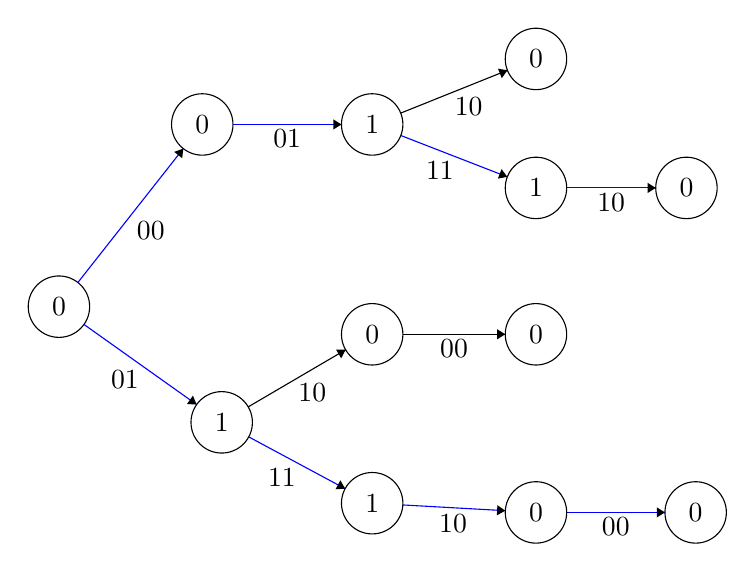
\begin{tikzpicture}[scale=0.13]
			\tikzstyle{every node}+=[inner sep=0pt]
			\draw [black] (6.3,-31.7) circle (3);
			\draw (6.3,-31.7) node {$0$};
			\draw [black] (20.3,-13.9) circle (3);
			\draw (20.3,-13.9) node {$0$};
			\draw [black] (22.2,-43) circle (3);
			\draw (22.2,-43) node {$1$};
			\draw [black] (36.9,-13.9) circle (3);
			\draw (36.9,-13.9) node {$1$};
			\draw [black] (36.9,-34.4) circle (3);
			\draw (36.9,-34.4) node {$0$};
			\draw [black] (36.9,-50.9) circle (3);
			\draw (36.9,-50.9) node {$1$};
			\draw [black] (52.9,-7.5) circle (3);
			\draw (52.9,-7.5) node {$0$};
			\draw [black] (52.9,-20.1) circle (3);
			\draw (52.9,-20.1) node {$1$};
			\draw [black] (67.6,-20.1) circle (3);
			\draw (67.6,-20.1) node {$0$};
			\draw [black] (52.9,-34.4) circle (3);
			\draw (52.9,-34.4) node {$0$};
			\draw [black] (52.9,-51.8) circle (3);
			\draw (52.9,-51.8) node {$0$};
			\draw [black] (68.5,-51.8) circle (3);
			\draw (68.5,-51.8) node {$0$};
			\draw [blue] (8.15,-29.34) -- (18.45,-16.26);
			\fill [black] (18.45,-16.26) -- (17.56,-16.58) -- (18.34,-17.2);
			\draw (13.87,-24.22) node [right] {$00$};
			\draw [blue] (8.75,-33.44) -- (19.75,-41.26);
			\fill [black] (19.75,-41.26) -- (19.39,-40.39) -- (18.81,-41.21);
			\draw (12.75,-37.85) node [below] {$01$};
			\draw [blue] (23.3,-13.9) -- (33.9,-13.9);
			\fill [black] (33.9,-13.9) -- (33.1,-13.4) -- (33.1,-14.4);
			\draw (28.6,-14.4) node [below] {$01$};
			\draw [black] (24.79,-41.49) -- (34.31,-35.91);
			\fill [black] (34.31,-35.91) -- (33.37,-35.89) -- (33.87,-36.75);
			\draw (31.05,-39.2) node [below] {$10$};
			\draw [blue] (24.84,-44.42) -- (34.26,-49.48);
			\fill [black] (34.26,-49.48) -- (33.79,-48.66) -- (33.32,-49.54);
			\draw (28.09,-47.45) node [below] {$11$};
			\draw [black] (39.69,-12.79) -- (50.11,-8.61);
			\fill [black] (50.11,-8.61) -- (49.19,-8.45) -- (49.56,-9.38);
			\draw (46.33,-11.23) node [below] {$10$};
			\draw [blue] (39.7,-14.98) -- (50.1,-19.02);
			\fill [black] (50.1,-19.02) -- (49.54,-18.26) -- (49.18,-19.19);
			\draw (43.51,-17.53) node [below] {$11$};
			\draw [blue] (55.9,-20.1) -- (64.6,-20.1);
			\fill [black] (64.6,-20.1) -- (63.8,-19.6) -- (63.8,-20.6);
			\draw (60.25,-20.6) node [below] {$10$};
			\draw [black] (39.9,-34.4) -- (49.9,-34.4);
			\fill [black] (49.9,-34.4) -- (49.1,-33.9) -- (49.1,-34.9);
			\draw (44.9,-34.9) node [below] {$00$};
			\draw [blue] (39.9,-51.07) -- (49.9,-51.63);
			\fill [black] (49.9,-51.63) -- (49.13,-51.09) -- (49.08,-52.09);
			\draw (44.8,-51.93) node [below] {$10$};
			\draw [blue] (55.9,-51.8) -- (65.5,-51.8);
			\fill [black] (65.5,-51.8) -- (64.7,-51.3) -- (64.7,-52.3);
			\draw (60.7,-52.3) node [below] {$00$};
		\end{tikzpicture}
	\end{center}
\end{frame}

\begin{frame}{A Better Graph Representation}
	\begin{center}
		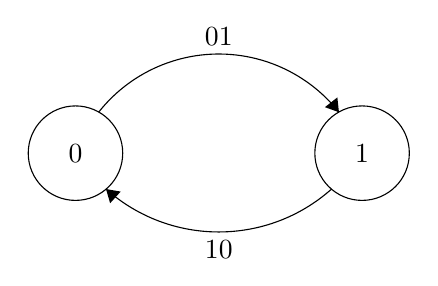
\begin{tikzpicture}[scale=0.2]
			\tikzstyle{every node}+=[inner sep=0pt]
			\draw [black] (23.9,-28.5) circle (3);
			\draw (23.9,-28.5) node {$0$};
			\draw [black] (42.1,-28.5) circle (3);
			\draw (42.1,-28.5) node {$1$};
			\draw [black] (25.371,-25.899) arc (141.67586:38.32414:9.725);
			\fill [black] (40.63,-25.9) -- (40.53,-24.96) -- (39.74,-25.58);
			\draw (33,-21.7) node [above] {$01$};
			\draw [black] (40.163,-30.779) arc (-48.33728:-131.66272:10.776);
			\fill [black] (25.84,-30.78) -- (26.1,-31.68) -- (26.77,-30.94);
			\draw (33,-34) node [below] {$10$};
		\end{tikzpicture}
	\end{center}
\end{frame}

\begin{frame}{A Better Graph Representation}
	\begin{center}
		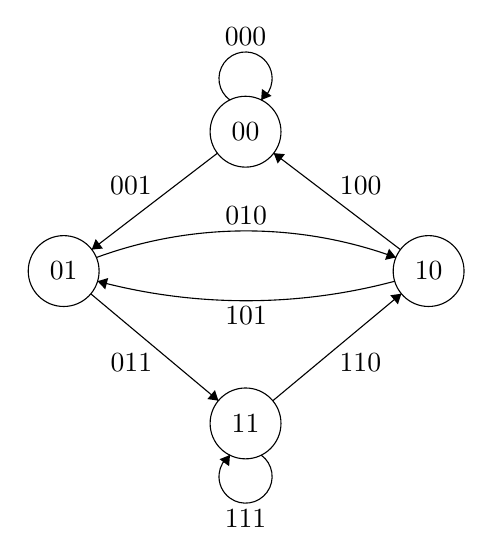
\begin{tikzpicture}[scale=0.15]
			\tikzstyle{every node}+=[inner sep=0pt]
			\draw [black] (41.6,-15.1) circle (3);
			\draw (41.6,-15.1) node {$00$};
			\draw [black] (26.2,-26.9) circle (3);
			\draw (26.2,-26.9) node {$01$};
			\draw [black] (57.1,-26.9) circle (3);
			\draw (57.1,-26.9) node {$10$};
			\draw [black] (41.6,-39.8) circle (3);
			\draw (41.6,-39.8) node {$11$};
			\draw [black] (40.277,-12.42) arc (234:-54:2.25);
			\draw (41.6,-7.85) node [above] {$000$};
			\fill [black] (42.92,-12.42) -- (43.8,-12.07) -- (42.99,-11.48);
			\draw [black] (39.22,-16.92) -- (28.58,-25.08);
			\fill [black] (28.58,-25.08) -- (29.52,-24.99) -- (28.91,-24.19);
			\draw (31.9,-20.5) node [above] {$001$};
			\draw [black] (28.5,-28.83) -- (39.3,-37.87);
			\fill [black] (39.3,-37.87) -- (39.01,-36.98) -- (38.37,-37.74);
			\draw (31.93,-33.84) node [below] {$011$};
			\draw [black] (43.91,-37.88) -- (54.79,-28.82);
			\fill [black] (54.79,-28.82) -- (53.86,-28.95) -- (54.5,-29.72);
			\draw (51.32,-33.84) node [below] {$110$};
			\draw [black] (54.71,-25.08) -- (43.99,-16.92);
			\fill [black] (43.99,-16.92) -- (44.32,-17.8) -- (44.93,-17);
			\draw (51.35,-20.5) node [above] {$100$};
			\draw [black] (42.923,-42.48) arc (54:-234:2.25);
			\draw (41.6,-47.05) node [below] {$111$};
			\fill [black] (40.28,-42.48) -- (39.4,-42.83) -- (40.21,-43.42);
			\draw [black] (28.971,-25.753) arc (110.15643:69.84357:36.795);
			\fill [black] (54.33,-25.75) -- (53.75,-25.01) -- (53.41,-25.95);
			\draw (41.65,-23) node [above] {$010$};
			\draw [black] (54.227,-27.763) arc (-75.0456:-104.9544:48.74);
			\fill [black] (29.07,-27.76) -- (29.72,-28.45) -- (29.97,-27.49);
			\draw (41.65,-29.91) node [below] {$101$};
		\end{tikzpicture}
	\end{center}
\end{frame}

\begin{frame}{De Bruijn Graph}
	Let $n \ge 1$.
	\pause
	$$
		V = \mathbb{F}_2^{n-1}
	$$
	\pause
	$$
		u \to v \text{ if } \emph{suffix}(u) = \emph{prefix}(v)
	$$
	\pause
	What graph problem are we solving?
\end{frame}

\begin{frame}{Eulerian Circuit}
	\begin{defn}[Circuit]
		A \emph{circuit} is a closed walk that uses an edge at most once.
	\end{defn}
	\pause
	\begin{defn}[Eulerian Circuit]
		A circuit is \emph{Eulerian} if it uses all edges exactly once.
	\end{defn}
\end{frame}

\begin{frame}{Eulerian Graphs}
	We say a (simple) (di)graph is Eulerian if it has an Eulerian circuit.
	\pause
	\begin{theorem}[Eulerian Graphs]
		$G$ is Eulerian if $\emph{indeg}(v) = \emph{outdeg}(v)$ for all $v \in V(G)$.
	\end{theorem}
\end{frame}

\begin{frame}{Eulerian Graphs Sufficiency}
	\begin{algo}
		\textul{\textsc{FindEulerianCircuit}($G$)}: \+
		\\ $T \gets$ maximal trail in $G$
		\\ $G' \gets G \setminus T$
		\\ $C \gets \textsc{FindEulerianCircuit}(G')$
		\\ return $T \cup C$
	\end{algo}
\end{frame}

\begin{frame}{Eulerian Graphs Sufficiency}
	\begin{proof}
		Suppose $G$ is balanced.
		\pause
		Then, $T$ must be a circuit.
		\pause
		$G'$ must be balanced.
		\pause
		Then, $T \cup C$ is Eulerian, by induction.
	\end{proof}

	\begin{claim}
		The above algorithm runs in $O(\abs{E})$ time.
	\end{claim}
\end{frame}

\begin{frame}{De Bruijn Sequences}
	\begin{claim}
		For all $n$, De Bruijn sequences exist.
	\end{claim}

	\begin{proof}
		Consider $G$, the De Bruijn graph.
		\pause
		For all $v \in V(G)$,
		$$
			\emph{indeg}(v) = \emph{outdeg}(v) = 2
		$$
		\pause
		Thus, $G$ is Eulerian.
	\end{proof}
\end{frame}

\begin{frame}{Additional Results}
	\begin{itemize}\onslide<+->
		\item There are $2^{2^{n-1} - n}$ such circular sequences \onslide<+->
		\item Considering not-circular, there are $2^{2^{n-1}}$ sequences \onslide<+->
		\item There is a bijection between pairs of De Bruijn sequences, and all binary $2^n$ sequences.
	\end{itemize}
\end{frame}

\section{De novo Genome Assembly}
\frame{\sectionpage}

\begin{frame}{Sequencing Is Hard}
	\begin{itemize}\onslide<+->
		\item First generation (Sanger) sequencing: Sorting Based \onslide<+->
		\item Next generation sequencing: Synthesis Based \onslide<+->
	\end{itemize}

	We get short $k$-mers, rather than long sequences.
\end{frame}

\begin{frame}{Problem Statement}
	There is a model string $T$.
	Given all $k$-mers, estimate $T$.
\end{frame}

\begin{frame}{Law of Assembly}
	If $\emph{suffix}(A) = \emph{prefix}(B)$, they might overlap.

	\pause
	$$
		\TA \TC \TG \cup \TC \TG \TT \implies \TA \TC \TG \TT
	$$
\end{frame}

\begin{frame}{Overlap Graphs (SCS)}
	Form a connected graph $G = K_n$.
	$$
		w(A, B) = \emph{suffix}(A) = \emph{prefix}(B)
	$$

	We want to find the shortest common superstring.
\end{frame}

\begin{frame}{Overlap Graphs (SCS)}
	\begin{center}
		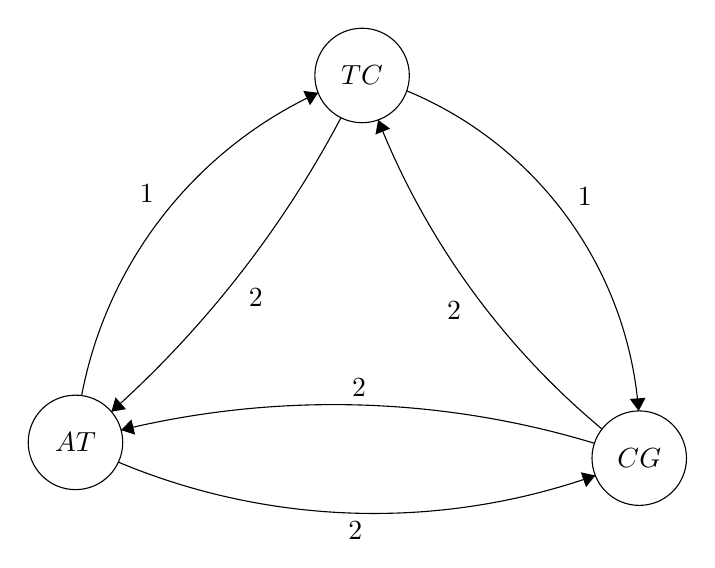
\begin{tikzpicture}[scale=0.2]
			\tikzstyle{every node}+=[inner sep=0pt]
			\draw [black] (35.1,-14.5) circle (3);
			\draw (35.1,-14.5) node {$TC$};
			\draw [black] (16.9,-37.8) circle (3);

			\draw (16.9,-37.8) node {$AT$};
			\draw [black] (52.7,-38.8) circle (3);
			\draw (52.7,-38.8) node {$CG$};
			\draw [black] (17.291,-34.827) arc (169.27925:114.73283:26.623);
			\fill [black] (32.31,-15.6) -- (31.37,-15.48) -- (31.79,-16.39);
			\draw (21.9,-21.98) node [left] {$1$};
			\draw [black] (37.936,-15.474) arc (67.46745:4.36266:23.984);

			\fill [black] (52.66,-35.8) -- (53.1,-34.97) -- (52.1,-35.04);
			\draw (48.76,-22.18) node [right] {$1$};

			\draw [black] (19.795,-37.015) arc (103.66146:73.13849:57.118);

			\fill [black] (19.8,-37.02) -- (20.69,-37.31) -- (20.45,-36.34);
			\draw (34.9,-34.89) node [above] {$2$};
			\draw [black] (49.91,-39.901) arc (-70.50928:-112.69077:42.098);
			\fill [black] (49.91,-39.9) -- (48.99,-39.7) -- (49.32,-40.64);
			\draw (34.67,-42.82) node [below] {$2$};
			\draw [black] (33.759,-17.183) arc (-27.8354:-48.15252:67.146);
			\fill [black] (19.18,-35.85) -- (20.11,-35.69) -- (19.44,-34.94);
			\draw (27.87,-28.58) node [right] {$2$};
			\draw [black] (50.337,-36.952) arc (-129.77958:-158.39031:49.049);
			\fill [black] (36.12,-17.32) -- (35.95,-18.25) -- (36.88,-17.88);
			\draw (41.41,-29.41) node [left] {$2$};
		\end{tikzpicture}
	\end{center}
\end{frame}

\begin{frame}{Overlap Graphs (SCS)}
	This is the \emph{Traveling Salesman Problem}.
	It is \emph{NP-Hard}

	\pause

	We may approximate with greedy Nearest Neighbor.
	This is a $\log n$ approximation.
\end{frame}

\begin{frame}{Additional Remarks}
	\begin{itemize}\onslide<+->
		\item Determining Overlaps: bloom filters \onslide<+->
		\item Tandem Repeats: $\TA\TA\TA\TA\TA$ \onslide<+->
	\end{itemize}
\end{frame}

\begin{frame}{De Bruijn Graphs}
	Break all $k$-mers into 2 $(k-1)$-mers.
	Create De Bruijn graph.

	\pause

	If the genome is $\TA\TA\TA\TT\TT\TT\TA$, for $k = 3$,
	\begin{center}
		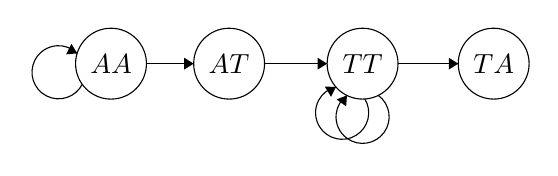
\begin{tikzpicture}[scale=0.15]
			\tikzstyle{every node}+=[inner sep=0pt]
			\draw [black] (17.1,-27) circle (3);
			\draw (17.1,-27) node {$AA$};
			\draw [black] (27.1,-27) circle (3);
			\draw (27.1,-27) node {$AT$};
			\draw [black] (38.4,-27) circle (3);
			\draw (38.4,-27) node {$TT$};
			\draw [black] (49.5,-27) circle (3);
			\draw (49.5,-27) node {$TA$};
			\draw [black] (20.1,-27) -- (24.1,-27);
			\fill [black] (24.1,-27) -- (23.3,-26.5) -- (23.3,-27.5);
			\draw [black] (14.669,-28.738) arc (-26.71222:-314.71222:2.25);
			\fill [black] (14.24,-26.13) -- (13.75,-25.32) -- (13.3,-26.21);
			\draw [black] (30.1,-27) -- (35.4,-27);
			\fill [black] (35.4,-27) -- (34.6,-26.5) -- (34.6,-27.5);
			\draw [black] (39.723,-29.68) arc (54:-234:2.25);

			\fill [black] (37.08,-29.68) -- (36.2,-30.03) -- (37.01,-30.62);
			\draw [black] (38.59,-29.982) arc (31.38014:-256.61986:2.25);
			\fill [black] (36.15,-28.96) -- (35.21,-28.95) -- (35.73,-29.81);
			\draw [black] (41.4,-27) -- (46.5,-27);
			\fill [black] (46.5,-27) -- (45.7,-26.5) -- (45.7,-27.5);
		\end{tikzpicture}
	\end{center}

	\pause

	We want to find an \emph{Eulerian Trail}.
\end{frame}

\begin{frame}{Additional Remarks}
	\begin{itemize}\onslide<+->
		\item Unequal coverage, repeats \onslide<+->
		\item Error correction, \onslide<+->
		\item Bubbles, islands
	\end{itemize}
\end{frame}

\begin{frame}{Brainteaser}
	\centering
	\includegraphics[width=\textwidth/2]{haruhi}
\end{frame}

\font\eightss=cmssq8
\font\eightssi=cmssqi8
\newcommand\quoteAuthorDate[3]{\begingroup
	\baselineskip 10pt
	\parfillskip 0pt
	\interlinepenalty 10000 % not needed in example
	\leftskip 0pt plus 40pc minus \parindent
	\let\rm=\eightss
	\let\sl=\eightssi
	\everypar{\sl}#1\par
	\nobreak\smallskip
	\noindent\rm--- #2\unskip\enspace(#3)\par
	\endgroup}
\begin{frame}
	\begin{center}
		\item \quoteAuthorDate{WAGA WAGA}{Sariel Har-Peled}{\textcolor{sigma@mainblue}{2024}}
	\end{center}
\end{frame}

\begin{frame}[allowframebreaks]{Bibliography}
	\bibliographystyle{alpha}
	\begin{itemize}
		\item Ben Langmea (JHU), \url{https://www.langmead-lab.org/teaching.html}
		\item Lionel Levine (MIT), \url{https://pi.math.cornell.edu/~levine/18.312/}
	\end{itemize}
\end{frame}

\end{document}
